\documentclass[../wstep.tex]{subfiles}

\begin{document}
\label{requirements:functional}

\subsection{Nadzorca}

\begin{figure}[H]
  \centering
  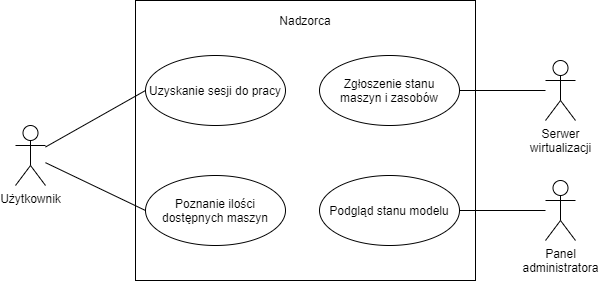
\includegraphics[width=\textwidth]{../diagrams/use_cases/overseer.png}
  \caption{Przypadki użycia aplikacji nadzorczej}
\end{figure}

\begin{table}[H]
  \caption[Przypadki użycia aplikacji nadzorczej]{Przypadki użycia aplikacji nadzorczej}
  \label{use-case-nadzorca}
  \centering
  \begin{tabular}{|p{0.07\textwidth}|p{0.17\textwidth}|p{0.25\textwidth}|p{0.375\textwidth}|}
    \hline Aktor                                                                    & Nazwa                             & Opis                                                               & Odpowiedź systemu                                                                                                                                                                                     \\ \hline
    \multirow{14}{=}{\rotatebox{90}{Użytkownik}}                                    & Uzyskanie sesji do pracy          & Uzyskanie sesji do pracy na maszynie wirtualnej odpowiedniego typu. & Użytkownikowi zostaje przydzielona maszyna wirtualna oraz zestawione połączenie RDP. Jeżeli przypisana do użytkownika sesja nie została jeszcze zakończona, to system przydziela mu tą samą maszynę. \\ \cline{2-4}
                                                                                    & Poznanie ilości dostępnych maszyn & Wyświetlanie szacowanej ilości dostępnych maszyn każdego typu.      & Użytkownikowi zostaje wyświetlona szacowana liczba dostępnych maszyn obliczona na podstawie informacji o~dostępnych zasobach każdego z~serwerów wirtualizacji. Zobaczy on ilość maszyn uruchomionych, zajętych przez niego oraz możliwych w~przyszłości do uruchomienia.                                        \\ \hline
    \multirow[b]{5}{=}{\rotatebox{90}{\parbox{1cm}{Serwer \newline wirtualizacji}}} & Zgłoszenie dostępnych zasobów     & Serwer zgłasza nadzorcy dostępne zasoby.                            & Nadzorca wykorzystuje zgłoszone zasoby do wyliczenia szacowanej liczby dostępnych maszyn oraz balansowania obciążeniem serwerów wirtualizacji.                                                        \\
    \hline
    \multirow[b]{5}{=}{\rotatebox{90}{\parbox{1cm}{Panel \newline administratora}}} & Podgląd stanu modelu              & Nadzorca udostępnia panelowi administratora stan zasobów systemu.  & Panel administratora wykorzystuje uzyskane dane to wyświetlenia administratorowi raportu o~stanie systemu.     \newline                                                                               \\
    \hline
  \end{tabular}
\end{table}


\subsection{Serwer wirtualizacji}

\begin{figure}[H]
  \centering
  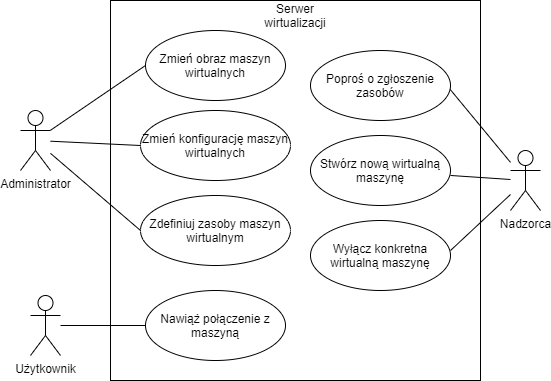
\includegraphics[width=\textwidth]{../diagrams/use_cases/virtualisation_server.png}
  \caption{Przypadki użycia serwera wirtualizacji}
\end{figure}


\begin{table}[H]
  \caption[Przypadki użycia serwera wirtualizacji]{Przypadki użycia serwera wirtualizacji}
  \label{use-case-virtsrv}
  \centering
  \begin{tabular}{|p{0.07\textwidth}|p{0.17\textwidth}|p{0.3\textwidth}|p{0.325\textwidth}|}
    \hline Aktor                                    & Nazwa                                 & Opis                                                                                                                       & Odpowiedź systemu                                                                                                                \\ \hline
    \multirow{6}{=}{\rotatebox{90}{Użytkownik}}     & Nawiązanie połączenia z~maszyną       & Użytkownik nawiązuje połączenie z~maszyną wirtualną.                                                                        & Maszyna wirtualna zostaje zajęta przez użytkownika; serwer wirtualizacji rozpoczyna monitorowanie, czy użytkownik nadal jest podłączony do maszyny. \\ \hline
    \multirow{14}{=}{\rotatebox{90}{Nadzorca}}      & Poproś o~zgłoszenie zasobów           & Nadzorca wysyła do wszystkich serwerów wirtualizacji prośbę o~zgłoszenie swoich używanych i~wolnych zasobów.                & Serwer wirtualizacji informuje nadzorcę o~stanie swoich zasobów.                                                                  \\ \cline{2-4}
                                                    & Stwórz nową maszynę wirtualną         & Nadzorca prosi serwer wirtualizacji o~stworzenie nowej maszyny wirtualnej dla danego użytkownika na wybranym typie maszyny. & Serwer wirtualizacji tworzy maszynę wirtualną wybranego typu i~udostępnia możliwość połączenia się z~nią.                         \\ \cline{2-4}
                                                    & Wyłącz konkretną maszynę wirtualną    & Nadzorca prosi serwer wirtualizacji aby wyłączył konkretną maszynę wirtualną.                                              & Serwer wirtualizacji wyłącza konkretną maszynę wirtualną oraz pilnuje aby na pewno się wyłączyła.                                \\ \hline
    \multirow{10}{=}{\rotatebox{90}{Administrator}} & Zmień obraz maszyn wirtualnych        & Zmiana obrazu źródłowego maszyn wirtualnych.                                                                                & Zdefiniowany przez administratora Vagrant Box jest używany przez serwery wirtualizacji.                                           \\ \cline{2-4}
                                                    & Zmień konfigurację maszyn wirtualnych & Zmiana zmiennej konfiguracji maszyn wirtualnych.                                                                            & Zmodyfikowany ansible playbook jest używany przez serwery wirtualizacji.                                                          \\ \cline{2-4}
                                                    & Zdefiniuj zasoby maszyn wirtualnych   & Zmiana łącznej ilości zasobów przeznaczonych na maszyny.                                                                    & Zmodyfikowana konfiguracja zasobów będzie wykorzystywana przez serwer wirtualizacji przy kolejnym uruchomieniu.                   \\
    \hline
  \end{tabular}
\end{table}

\subsection{Panel administratora}

\begin{figure}[H]
  \centering
  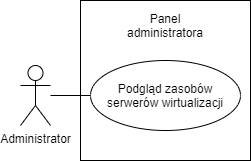
\includegraphics[width=0.4\textwidth]{../diagrams/use_cases/admin_panel.png}
  \caption{Przypadki użycia panelu administratora}
\end{figure}

\begin{table}[H]
  \caption[Przypadki użycia panelu administratora]{Przypadki użycia panelu administratora}
  \label{use-case-admin-panel}
  \centering
  \begin{tabular}{|p{0.07\textwidth}|p{0.17\textwidth}|p{0.25\textwidth}|p{0.375\textwidth}|}
    \hline Aktor                                   & Nazwa                                  & Opis                                                              & Odpowiedź systemu                                                                                                                         \\ \hline
    \multirow{5}{=}{\rotatebox{90}{Administrator}} & Podgląd zasobów serwerów wirtualizacji & Wyświetlanie wolnych oraz zajętych zasobów serwerów wirtualizacji. & Wyświetlenie zasobów poszczególnych serwerów wirtualizacji, liczby zajętych maszyn oraz szacowanej liczby wolnych maszyn. \newline \\
    \hline
  \end{tabular}
\end{table}

\end{document}